\documentclass{fkssolpub}

\usepackage[czech]{babel}
\usepackage{fontspec}
\usepackage{fkssugar}
\usepackage{amsmath}
\usepackage{graphicx}

\author{Ondřej Sedláček}
\school{Gymnázium Oty Pavla} 
\series{2}
\problem{D} 

\renewcommand{\angle}{\sphericalangle}

\begin{document}

\begin{figure}
	\begin{center}
		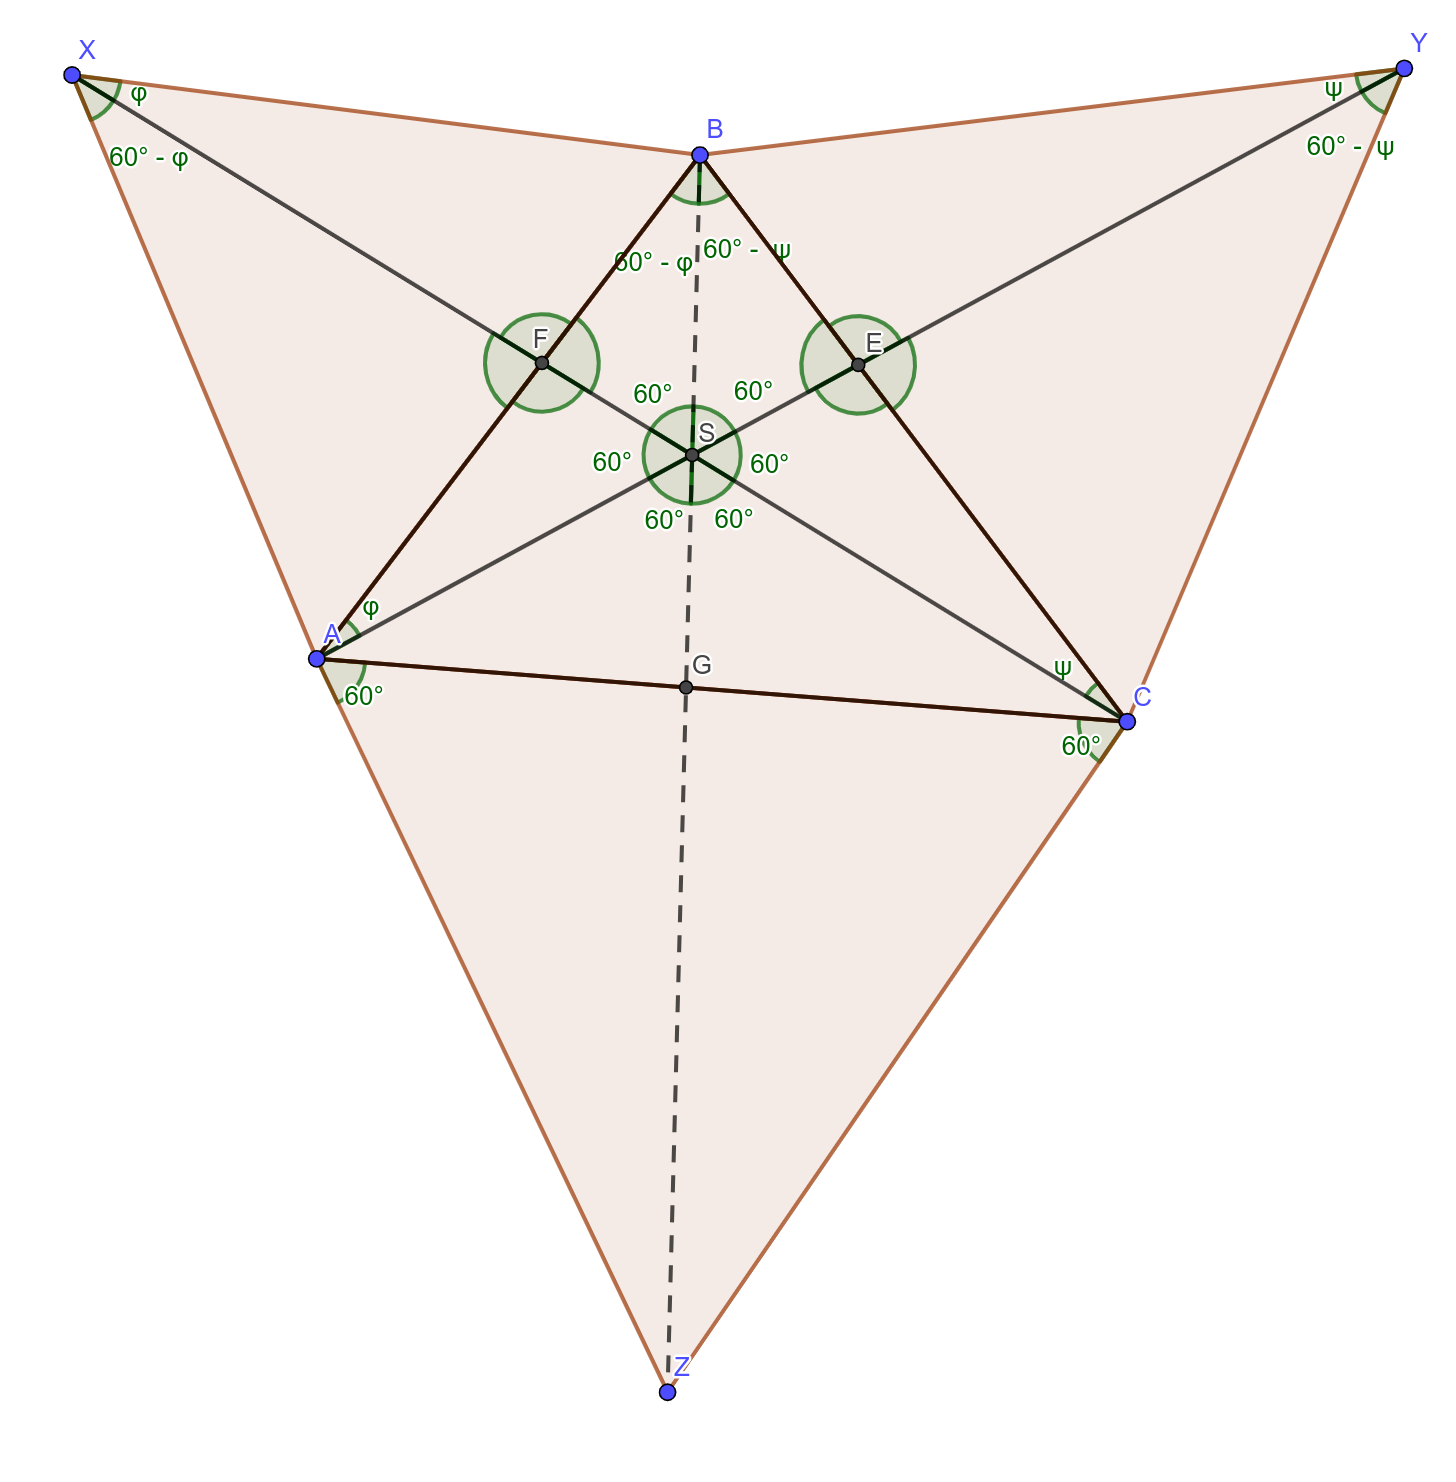
\includegraphics[width=0.85\textwidth]{D-fig}
	\end{center}
	\caption{Konstrukce úlohy s vyznačenými úhly}
	\label{fig:1}
\end{figure}

V zadání po nás chtějí, abychom dokázali, že se úsečky $AY$,$BZ$,$CX$ protínají v jednom bodě. Tehdy ale tento průsečík musí být vevnitř trojúhelníku $ABC$, což ale není v některých konfiguracích pravda. Proto po zbytek úlohy budu předpokládat, že dvě z těchto úseček mají průsečík vevnitř trojúhelníku.

Nechť průsečík $AY$ a $CX$ je $S$. Díky připsaným rovnostranným trojúhelníkům platí, že $BXC$ a $BAY$ jsou shodné trojúhelníky, proto tehdy $|\angle BXC| = |\angle BAY| = \phi$ a $|\angle XCB| = |\angle BYA| = \psi$. Pak podle věty uu platí $FBX \sim FSA$ a $EYB \sim ECS$, proto $|\angle ASF| = |\angle ESC| = 60^{\circ}$. Tedy aby bod $S$ byl vevnitř trojúhelníku, každý úhel trojúhelníku $ABC$ je menší než $120 ^{\circ}$. Pokud ale BÚNO platí, že $|\angle ABC| = 120^{\circ}$, pak $B = S$ a tím pádem se úsečky nutně protnou v bodě $B$.

Z podobnosti $FBX \sim FSA$, víme, že $\frac{|BF|}{|FS|} = \frac{|XF|}{|FA|}$ a tedy $\frac{|BF|}{|XF|} = \frac{|FS|}{|FA|}$. A protože $|\angle XFA| = |\angle BFS|$, podle věty sus platí $FXA \sim FBS$. Analogicky dokážeme i podobnost $ECY \sim ESB$. Z těchto podobností pak zjistíme velikosti úhlů $|\angle FSB| = |\angle BSE| = 60 ^{\circ}$.

Teď nám tedy zbývá zjistit velikosti úhlů $|\angle CSZ|$ a $|\angle ZSA|$. Ze zbývajících úhlů s vrcholem v $S$ dopočítáme $|\angle CSA| = 120^{\circ}$. A protože $|\angle AZC| = 60^{\circ}$, čtyřúhelník $SAZC$ je tětivový, proto $|\angle CAZ| = |\angle CSZ| = 60^{\circ}$ a $|\angle ZCA| = |\angle ZSA| = 60^{\circ}$.

A poněvadž nám vyšlo, že $|\angle BSZ| = |\angle BSE| + |\angle ESC| + |\angle CSZ| = 180^{\circ}$, bod $S$ leží na úsečce $BZ$ a tedy všechny úsečky se protínají v jednom bodě. Protože ve zbývajících konfiguracích se některé z těchto úseček neprotnou vůbec, je tímto důkaz u konce.

\end{document}
